% I seguenti commenti speciali impostano:
% 1.
% 2. PDFLaTeX come motore di composizione;
% 3. tesi.tex come documento principale;
% 4. il controllo ortografico italiano per l'editor.

% !TEX encoding = UTF-8
% !TEX TS-program = pdflatex
% !TEX root = tesi.tex
% !TeX spellcheck = de_DE

\documentclass[10pt,                    % corpo del font principale
               a4paper,                 % carta A4
               twoside,                 % impagina per fronte-retro
               openright,               % inizio capitoli a destra
               english,
               italian,
               ]{book}

\usepackage[utf8]{inputenc}             % codifica di input; anche [latin1] va bene
                                        % NOTA BENE! va accordata con le preferenze dell'editor

%**************************************************************
% Importazione package
%**************************************************************

%\usepackage{amsmath,amssymb,amsthm}    % matematica

\usepackage[english, italian]{babel}    % per scrivere in italiano e in inglese;
                                        % l'ultima lingua (l'italiano) risulta predefinita

\usepackage{bookmark}                   % segnalibri

\usepackage{caption}                    % didascalie

\usepackage{chngpage,calc}              % centra il frontespizio

\usepackage{csquotes}                   % gestisce automaticamente i caratteri (")

\usepackage{emptypage}                  % pagine vuote senza testatina e piede di pagina

\usepackage{epigraph}					% per epigrafi

\usepackage{eurosym}                    % simbolo dell'euro

\usepackage[T1]{fontenc}                % codifica dei font:
                                        % NOTA BENE! richiede una distribuzione *completa* di LaTeX

%\usepackage{indentfirst}               % rientra il primo paragrafo di ogni sezione

\usepackage{graphicx}                   % immagini

\usepackage{hyperref}                   % collegamenti ipertestuali



\usepackage[binding=5mm]{layaureo}      % margini ottimizzati per l'A4; rilegatura di 5 mm

\usepackage{listings}                   % codici

\usepackage{microtype}                  % microtipografia

\usepackage{mparhack,fixltx2e,relsize}  % finezze tipografiche

\usepackage{nameref}                    % visualizza nome dei riferimenti

\usepackage[font=small]{quoting}        % citazioni

\usepackage{subfig}                     % sottofigure, sottotabelle

\usepackage[italian]{varioref}          % riferimenti completi della pagina

\usepackage[dvipsnames]{xcolor}         % colori

\usepackage{booktabs}                   % tabelle
\usepackage{tabularx}                   % tabelle di larghezza prefissata
\usepackage{longtable}                  % tabelle su più pagine
\usepackage{ltxtable}                   % tabelle su più pagine e adattabili in larghezza

\usepackage[toc, acronym]{glossaries}   % glossario
                                        % per includerlo nel documento bisogna:
                                        % 1. compilare una prima volta tesi.tex;
                                        % 2. eseguire: makeindex -s tesi.ist -t tesi.glg -o tesi.gls tesi.glo
                                        % 3. eseguire: makeindex -s tesi.ist -t tesi.alg -o tesi.acr tesi.acn
                                        % 4. compilare due volte tesi.tex.

\usepackage[backend=biber,style=verbose-ibid,hyperref,backref]{biblatex}
                                        % eccellente pacchetto per la bibliografia;
                                        % produce uno stile di citazione autore-anno;
                                        % lo stile "numeric-comp" produce riferimenti numerici
                                        % per includerlo nel documento bisogna:
                                        % 1. compilare una prima volta tesi.tex;
                                        % 2. eseguire: biber tesi
                                        % 3. compilare ancora tesi.tex.
\usepackage{url}
\usepackage{array} % Improves `tabular` and `array` environments
\usepackage{pict2e} % Allows \linethickness{...} in diagonal lines
\usepackage{slashbox} % Defines \backslashbox{..}{..}
\usepackage{xcolor}

%**************************************************************
% file contenente le impostazioni della tesi
%**************************************************************

%**************************************************************
% Frontespizio
%**************************************************************

% Autore
\newcommand{\myName}{Mauro Carlin 1184446\\ Mattia Bottaro 1179480}                                    
\newcommand{\myTitle}{Titolo della tesi}

% Tipo di tesi                   
\newcommand{\myDegree}{Tesi di laurea triennale}

% Università             
\newcommand{\myUni}{Università degli Studi di Padova}

% Facoltà       
\newcommand{\myFaculty}{Corso di Laurea Magistrale in Informatica}

% Dipartimento
\newcommand{\myDepartment}{Dipartimento di Matematica "Tullio Levi-Civita"}

% Luogo
\newcommand{\myLocation}{Padova}

% Anno accademico
\newcommand{\myAA}{2017-2018}


%**************************************************************
% Impostazioni di impaginazione
% see: http://wwwcdf.pd.infn.it/AppuntiLinux/a2547.htm
%**************************************************************

\setlength{\parindent}{14pt}   % larghezza rientro della prima riga
\setlength{\parskip}{0pt}   % distanza tra i paragrafi


%**************************************************************
% Impostazioni di biblatex
%**************************************************************
\bibliography{bibliografia} % database di biblatex 

\defbibheading{bibliography} {
    \cleardoublepage
    \phantomsection 
    \addcontentsline{toc}{chapter}{\bibname}
    \chapter*{\bibname\markboth{\bibname}{\bibname}}
}

\setlength\bibitemsep{1.5\itemsep} % spazio tra entry

\DeclareBibliographyCategory{opere}
\DeclareBibliographyCategory{web}

\addtocategory{opere}{womak:lean-thinking}
\addtocategory{web}{site:agile-manifesto}

\defbibheading{opere}{\section*{Riferimenti bibliografici}}
\defbibheading{web}{\section*{Siti Web consultati}}


%**************************************************************
% Impostazioni di caption
%**************************************************************
\captionsetup{
    tableposition=top,
    figureposition=bottom,
    font=small,
    format=hang,
    labelfont=bf
}


%**************************************************************
% Impostazioni di graphicx
%**************************************************************
\graphicspath{{immagini/}} % cartella dove sono riposte le immagini


%**************************************************************
% Impostazioni di hyperref
%**************************************************************
\hypersetup{
    %hyperfootnotes=false,
    %pdfpagelabels,
    %draft,	% = elimina tutti i link (utile per stampe in bianco e nero)
    colorlinks=true,
    linktocpage=true,
    pdfstartpage=1,
    pdfstartview=FitV,
    % decommenta la riga seguente per avere link in nero (per esempio per la stampa in bianco e nero)
    %colorlinks=false, linktocpage=false, pdfborder={0 0 0}, pdfstartpage=1, pdfstartview=FitV,
    breaklinks=true,
    pdfpagemode=UseNone,
    pageanchor=true,
    pdfpagemode=UseOutlines,
    plainpages=false,
    bookmarksnumbered,
    bookmarksopen=true,
    bookmarksopenlevel=1,
    hypertexnames=true,
    pdfhighlight=/O,
    %nesting=true,
    %frenchlinks,
    urlcolor=webbrown,
    linkcolor=RoyalBlue,
    citecolor=webgreen,
    %pagecolor=RoyalBlue,
    %urlcolor=Black, linkcolor=Black, citecolor=Black, %pagecolor=Black,
    pdftitle={\myTitle},
    pdfauthor={\textcopyright\ \myName, \myUni, \myFaculty},
    pdfsubject={},
    pdfkeywords={},
    pdfcreator={pdfLaTeX},
    pdfproducer={LaTeX}
}

%**************************************************************
% Impostazioni di itemize
%**************************************************************
\renewcommand{\labelitemi}{$\ast$}

%\renewcommand{\labelitemi}{$\bullet$}
%\renewcommand{\labelitemii}{$\cdot$}
%\renewcommand{\labelitemiii}{$\diamond$}
%\renewcommand{\labelitemiv}{$\ast$}


%**************************************************************
% Impostazioni di listings
%**************************************************************
\lstset{
    language=[LaTeX]Tex,%C++,
    keywordstyle=\color{RoyalBlue}, %\bfseries,
    basicstyle=\small\ttfamily,
    %identifierstyle=\color{NavyBlue},
    commentstyle=\color{Green}\ttfamily,
    stringstyle=\rmfamily,
    numbers=none, %left,%
    numberstyle=\scriptsize, %\tiny
    stepnumber=5,
    numbersep=8pt,
    showstringspaces=false,
    breaklines=true,
    frameround=ftff,
    frame=single
} 


%**************************************************************
% Impostazioni di xcolor
%**************************************************************
\definecolor{webgreen}{rgb}{0,.5,0}
\definecolor{webbrown}{rgb}{.6,0,0}


%**************************************************************
% Altro
%**************************************************************

\newcommand{\omissis}{[\dots\negthinspace]} % produce [...]

% eccezioni all'algoritmo di sillabazione
\hyphenation
{
    ma-cro-istru-zio-ne
    gi-ral-din
}

\newcommand{\sectionname}{sezione}
\addto\captionsitalian{\renewcommand{\figurename}{Figura}
                       \renewcommand{\tablename}{Tabella}}

\newcommand{\glsfirstoccur}{\ap{{[g]}}}

\newcommand{\intro}[1]{\emph{\textsf{#1}}}

%**************************************************************
% Environment per ``rischi''
%**************************************************************
\newcounter{riskcounter}                % define a counter
\setcounter{riskcounter}{0}             % set the counter to some initial value

%%%% Parameters
% #1: Title
\newenvironment{risk}[1]{
    \refstepcounter{riskcounter}        % increment counter
    \par \noindent                      % start new paragraph
    \textbf{\arabic{riskcounter}. #1}   % display the title before the 
                                        % content of the environment is displayed 
}{
    \par\medskip
}

\newcommand{\riskname}{Rischio}

\newcommand{\riskdescription}[1]{\textbf{\\Descrizione:} #1.}

\newcommand{\risksolution}[1]{\textbf{\\Soluzione:} #1.}

%**************************************************************
% Environment per ``use case''
%**************************************************************
\newcounter{usecasecounter}             % define a counter
\setcounter{usecasecounter}{0}          % set the counter to some initial value

%%%% Parameters
% #1: ID
% #2: Nome
\newenvironment{usecase}[2]{
    \renewcommand{\theusecasecounter}{\usecasename #1}  % this is where the display of 
                                                        % the counter is overwritten/modified
    \refstepcounter{usecasecounter}             % increment counter
    \vspace{10pt}
    \par \noindent                              % start new paragraph
    {\large \textbf{\usecasename #1: #2}}       % display the title before the 
                                                % content of the environment is displayed 
    \medskip
}{
    \medskip
}

\newcommand{\usecasename}{UC}

\newcommand{\usecaseactors}[1]{\textbf{\\Attori Principali:} #1. \vspace{4pt}}
\newcommand{\usecasepre}[1]{\textbf{\\Precondizioni:} #1. \vspace{4pt}}
\newcommand{\usecasedesc}[1]{\textbf{\\Descrizione:} #1. \vspace{4pt}}
\newcommand{\usecasepost}[1]{\textbf{\\Postcondizioni:} #1. \vspace{4pt}}
\newcommand{\usecasealt}[1]{\textbf{\\Scenario Alternativo:} #1. \vspace{4pt}}

%**************************************************************
% Environment per ``namespace description''
%**************************************************************

\newenvironment{namespacedesc}{
    \vspace{10pt}
    \par \noindent                              % start new paragraph
    \begin{description} 
}{
    \end{description}
    \medskip
}

\newcommand{\classdesc}[2]{\item[\textbf{#1:}] #2}                     % file con le impostazioni personali

\begin{document}
%**************************************************************
% Materiale iniziale
%**************************************************************
\frontmatter
% !TEX encoding = UTF-8
% !TEX TS-program = pdflatex
% !TEX root = ../tesi.tex

%**************************************************************
% Frontespizio 
%**************************************************************
\begin{titlepage}

\begin{center}

\begin{LARGE}
\textbf{\myUni}\\
\end{LARGE}

\vspace{10pt}

\begin{Large}
\textsc{\myDepartment}\\
\end{Large}

\vspace{10pt}

\begin{large}
\textsc{\myFaculty}\\
\end{large}

\vspace{30pt}
\begin{figure}[htbp]
\begin{center}

\includegraphics[height=6cm]{logo-unipd}
\end{center}
\end{figure}
\vspace{30pt} 

\begin{LARGE}
\begin{center}
\textbf{Un'intelligenza artificiale per risolvere \\IQ Puzzler}\\
\end{center}
\end{LARGE}

\vspace{40pt} 

\begin{Large}
\begin{center}
\textit{Studenti}\\ 
\vspace{10pt} 
\myName
\end{center}
\end{Large}

\vspace{40pt}

\line(1, 0){338}
\begin{normalsize}
\textsc{Anno Accademico \myAA}
\end{normalsize}

\end{center}
\end{titlepage} 
% !TEX encoding = UTF-8
% !TEX TS-program = pdflatex
% !TEX root = ../tesi.tex

%**************************************************************
% Indici
%**************************************************************
\cleardoublepage
\pdfbookmark{\contentsname}{tableofcontents}
\setcounter{tocdepth}{2}
\tableofcontents
%\markboth{\contentsname}{\contentsname} 
\clearpage

\begingroup 
    \let\clearpage\relax
    \let\cleardoublepage\relax
    \let\cleardoublepage\relax
    %*******************************************************
    % Elenco delle figure
    %*******************************************************    
    \phantomsection
    \pdfbookmark{\listfigurename}{lof}
    \listoffigures

    \vspace*{8ex}

    %*******************************************************
    % Elenco delle tabelle
    %*******************************************************
    \phantomsection
    \pdfbookmark{\listtablename}{lot}
    \listoftables
        
    \vspace*{8ex}
\endgroup

\cleardoublepage


%**************************************************************
% Materiale principale
%**************************************************************
\mainmatter
% !TeX spellcheck = de_DE
% !TEX encoding = UTF-8
% !TEX TS-program = pdflatex
% !TEX root = ../tesi.tex

%**************************************************************
\chapter{Introduzione}
\label{cap:introduzione}
%**************************************************************
\section{Descrizione IQ Puzzler}
Lo scopo di IQ Puzzler è quello di riempire la griglia di gioco con tutte le varie forme a disposizione. Queste forme sono di varia dimensione, colore e struttura, e possono essere combinate in diversi modi per completare la griglia.\\
Il gioco comprende anche 100 configurazioni iniziali, dove alcune forme sono già posizionate all'interno della griglia e solo le rimanenti devono essere piazzate. All'aumentare delle forme rimanenti, aumenta notevolmete la complessità del gioco.\\ 
\begin{figure}[h]
	\centering
	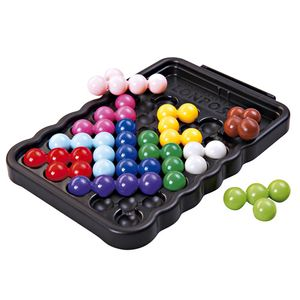
\includegraphics[scale=0.5]{immagini/iqpuzzler}
	\caption{Le forme di gioco di IQ Puzzler.}
	\label{fig:iqpuzzler}
\end{figure}

\newpage
\subsection{Forme di gioco}
Le forme totali sono 11, ognuna con una propria struttura diversa dalle altre, e sono formate da dei pallini collegati in modo da essere inseriti nelle celle della griglia.

\begin{figure}[h]
	
	\begin{minipage}{3.5cm}
		\centering
		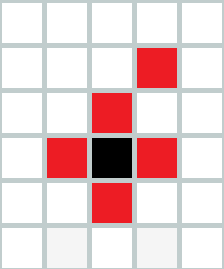
\includegraphics[scale=0.30]{immagini/p}
		\caption{}
		\label{p}
	\end{minipage}
	\ \hspace{2mm} \hspace{3mm} \
	\begin{minipage}{3.5cm}
		\centering
		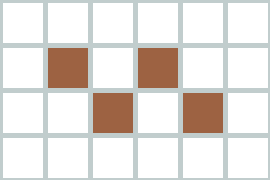
\includegraphics[scale=0.30]{immagini/z}
		\caption{}
		\label{z}
	\end{minipage}
	\ \hspace{2mm} \hspace{3mm} \
	\begin{minipage}{3.5cm}
		\centering
		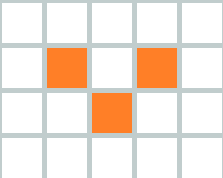
\includegraphics[scale=0.30]{immagini/smallv}
		\caption{}
		\label{smallv}
	\end{minipage}
\end{figure}

\begin{figure}[h]
	
	\begin{minipage}{3.5cm}
		\centering
		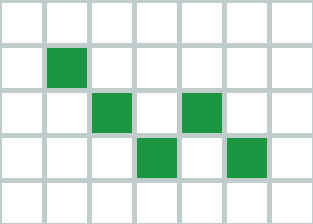
\includegraphics[scale=0.30]{immagini/bigz}
		\caption{}
		\label{bigz}
	\end{minipage}
	\ \hspace{2mm} \hspace{3mm} \
	\begin{minipage}{3.5cm}
		\centering
		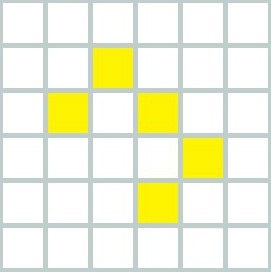
\includegraphics[scale=0.25]{immagini/yellow}
		\caption{}
		\label{c}
	\end{minipage}
	\ \hspace{2mm} \hspace{3mm} \
	\begin{minipage}{3.5cm}
		\centering
		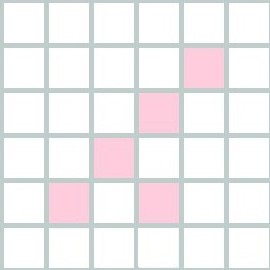
\includegraphics[scale=0.25]{immagini/Y}
		\caption{}
		\label{y}
	\end{minipage}
\end{figure}

\begin{figure}[h]
	
	\begin{minipage}{3.5cm}
		\centering
		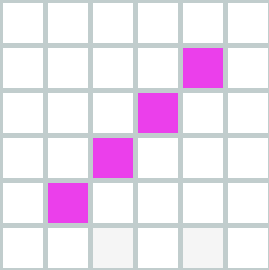
\includegraphics[scale=0.30]{immagini/i}
		\caption{}
		\label{i}
	\end{minipage}
	\ \hspace{2mm} \hspace{3mm} \
	\begin{minipage}{3.5cm}
		\centering
		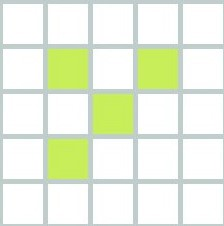
\includegraphics[scale=0.25]{immagini/T}
		\caption{}
		\label{t}
	\end{minipage}
	\ \hspace{2mm} \hspace{3mm} \
	\begin{minipage}{3.5cm}
		\centering
		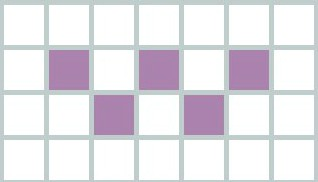
\includegraphics[scale=0.25]{immagini/w}
		\caption{}
		\label{w}
	\end{minipage}
\end{figure}

\begin{figure}[h]
	\centering
	\begin{minipage}{3.5cm}
		\centering
		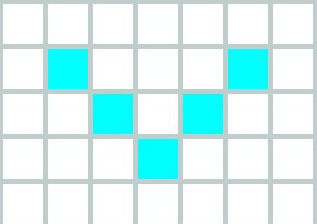
\includegraphics[scale=0.25]{immagini/v}
		\caption{}
		\label{v}
	\end{minipage}
	\ \hspace{2mm} \hspace{3mm} \
	\begin{minipage}{3.5cm}
		\centering
		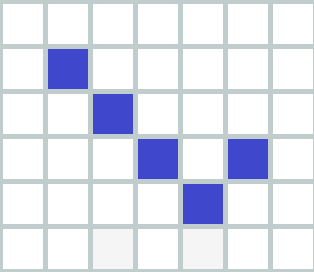
\includegraphics[scale=0.30]{immagini/L}
		\caption{}
		\label{l}
	\end{minipage}
\end{figure}

\newpage
\subsection{Griglia di gioco}
La griglia è formata da 11 righe con 4 o 5 celle, dove ogni cella è collegata solo con quelle nelle sue 2 diagonali. In totale la griglia è formata da 50 celle.

\begin{figure}[h]
	\centering
	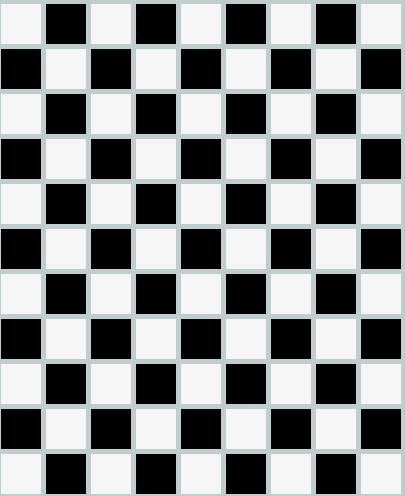
\includegraphics[scale=0.3]{immagini/griglia}
	\caption{La griglia di gioco di IQ Puzzler. Le forme possono essere piazzate utilizzando solo le celle bianche.}
	\label{fig:griglia}
\end{figure}


\newpage
\section{Scopo del progetto}
Lo scopo del nostro progetto è stato quello di ricreare questo gioco ed implementare alcuni dei metodi risolutivi visti durante il corso di Intelligenza Artificiale per risolverlo. \\
In un secondo momento abbiamo confrontato le performance dei vari algoritmi in modo da valutare la loro efficienza rispetto a questo problema.

\section{PEAS}

\subsection{Performance measure}
\label{performance}
La misura di performance è il tempo impiegato da un algoritmo per risolvere il problema a partire da una delle configurazioni iniziali. Oltre al tempo, abbiamo anche considerato il numero di azioni necessarie per raggiungere una soluzione, in maniera tale da poter fare osservazioni più precise su alcuni tipi di solver.\\
Tuttavia, la misura di performance più importante rimane la prima.

\subsection{Environment}
Il gioco analizzato presenta un ambiente totalmente osservabile, deterministico, sequenziale, statico, discreto e single-agent.  L'ambiente è completamente determinato dallo stato corrente e dall'agente che può effettuare una sola mossa alla volta.
L'azione dell'agente determina le azioni future dato che il possibile cammino
si riduce ad ogni passo.

\subsection{Actuators}
Il programma rappresenta l'esecuzione di un'azione attraverso la colorazione delle celle assegnate ad una determinata forma (passo di computazione).

\subsection{Sensors}
Ad ogni passo di computazione l'input della funzione agente è rappresentato dalla griglia e dalle forme rimanenti da inserire.

\section{Formalizzazione del problema}
\begin{itemize}
	\item \textbf{Stato inziale}: configurazione iniziale (possibilmente anche vuota) della griglia e relative forme mancanti da inserire;
	\item \textbf{Azioni possibili}: tutti i possibili modi di inserire una forma non ancora presente nella griglia;
	\item \textbf{Transition model}: colorazione, a seconda del colore della forma, della posizione scelta nella griglia;
	\item \textbf{Test obiettivo}: controllare se tutte le forme sono state inserite nella griglia, in modo da riempirla completamente;
	\item \textbf{Path cost}: tempo necessario per raggiungere la soluzione.
					
\end{itemize}

\section{Strumenti utilizzati}
Il programma è stato completamente sviluppato in Python 3.6 con l'utilizzo della libreria \textit{pygame} per quanto rigurda la parte grafica, e la libreria \textit{python-constraint} per la risoluzione del problema formulato come CSP. \\
La libreria \textit{python-constraint} è stata inoltre modificata e inclusa nella cartella \texttt{pythonConstraint/} per due motivi:
\begin{itemize}
	\item apportare delle migliorie agli algoritmi presenti, che verranno esposte successivamente nel documento;
	\item permettere di visualizzare ogni assegnamento parziale durante l'esecuzione dell'algoritmo.
\end{itemize}  

\section{Utilizzo del programma}
Per poter utilizzare il programma è necessario:
\begin{itemize}
	\item aver installato nel computer Python 3;
	\item spostarsi con il terminale alla cartella radice (\texttt{IQPuzzlerSoler/}) contenente il programma;
	\item eseguire uno di questi due comandi:
	\begin{itemize}
		\item \begin{verbatim}
		python main.py
		\end{verbatim}inizia l'esecuzione del programma, guidando l'utente nella scelta della difficoltà del problema e in che modo risolverlo. Le possibili difficoltà sono 5 (da 0 a 4) e di complessità crescente. I metodi di risoluzione sono quattro, tre dei quali con una variante ...
		\item \begin{verbatim}
		sh Test/scriptTest.sh
		\end{verbatim}esegue automaticamente una serie di esempi di problemi con vari metodi di risoluzione, tracciando i risultati ottenuti nel file \texttt{Test/testResult.txt}. 
	\end{itemize}
\end{itemize}
\begin{figure}[h]
	\centering
	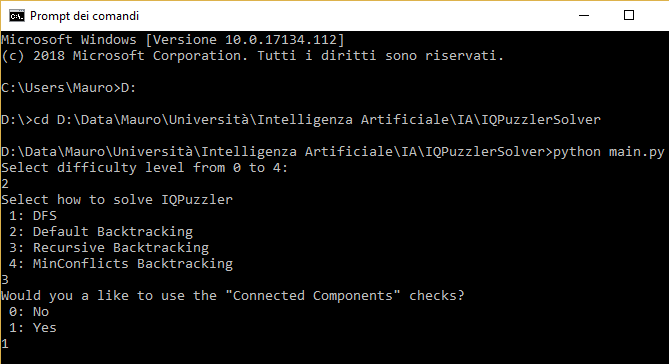
\includegraphics[scale=0.65]{immagini/exe}
	\caption{Esempio di esecuzione del programma}
	\label{fig:exe}
\end{figure}


             % Introduzione
% !TEX encoding = UTF-8
% !TEX TS-program = pdflatex
% !TEX root = ../tesi.tex

%**************************************************************
\chapter{Metodi di risoluzione}
\label{cap:algoritmi}
%**************************************************************

\section{DFS}
\subsection{Descrizione}
Il primo algoritmo utilizzato per risolvere il nostro problema è stato il Depth First Search. È una strategia di ricerca non informata in quanto non si utilizzano informazioni aggiuntive sugli stati oltre alla definizione iniziale del problema.
Quindi l'algoritmo è solamente in grado di generare successori e distinguere se sono uno stato obiettivo o meno. \\
Questa strategia esplora tutti gli stati dell'albero di ricerca in profondità, cioè espande prima lo stato più profondo non ancora esplorato, ritornando indietro nel caso il cammino non porti a nessuno stato obiettivo in un numero finito di azioni. \\
Questo tipo di ricerca termina non appena trova il primo stato obiettivo, generando però, nel caso pessimo, una complessità temporale (numero di stati generati) di $\mathcal{O}(b^m)$ dove m è la massima lunghezza di un percorso e b il massimo numero di successori di uno stato, rendendo questo algoritmo poco efficiente.
\begin{figure}[h]
	\centering
	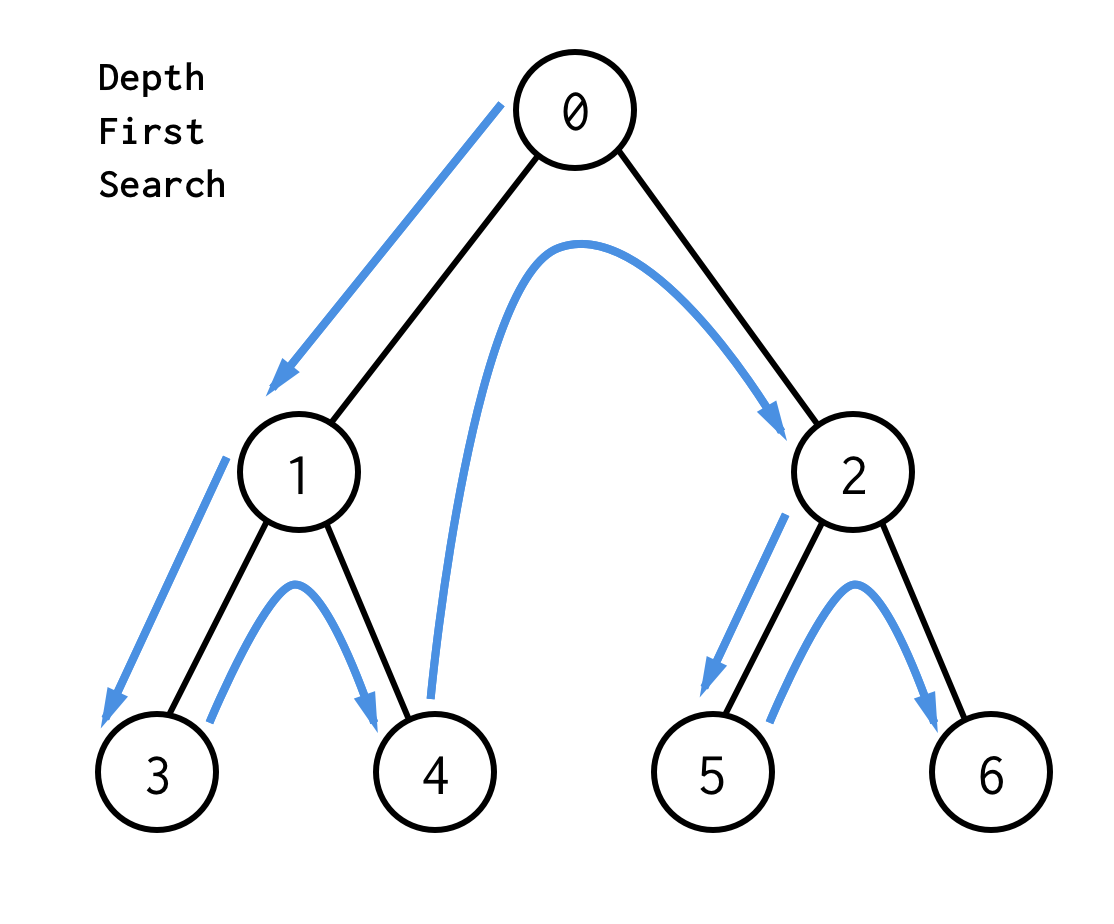
\includegraphics[scale=0.25]{immagini/dfs}
	\caption{Esempio di ricerca DFS}
	\label{fig:dfs}
\end{figure}

\subsection{Utilizzo}
Nel nostro caso l'algoritmo DFS è stato implementato in maniera ricorsiva, dove ogni stato rappresenta la configurazione attuale della griglia, intesa come forme già inserite e la loro posizione (coordinate all'interno della griglia). La configurazione iniziale della griglia rappresenta lo stato iniziale dal quale iniziale la ricerca in profondità.\\
I successori di ogni stato sono tutti i possibili posizionamenti, consistenti con l'assegnamento corrente (forme inserite e relativa posizione nella griglia), delle forme non ancora presenti nella griglia di gioco. Quindi l'algoritmo ad ogni passo sceglie la prossima forma da inserire, assegnandole il primo valore consistente nel suo dominio.
Qualora non ce ne fossero si ritorna allo stato precedente, espandendo un altro successore, fino ad arrivare ad uno stato obiettivo dove tutte le forme sono piazzate all'interno della griglia, in modo da riempirla totalmente.  \\
Essendo il nostro spazio di ricerca finito, l'algoritmo DFS ci assicura di ritornare sempre una soluzione al problema.
\begin{figure}[h]
	\centering
	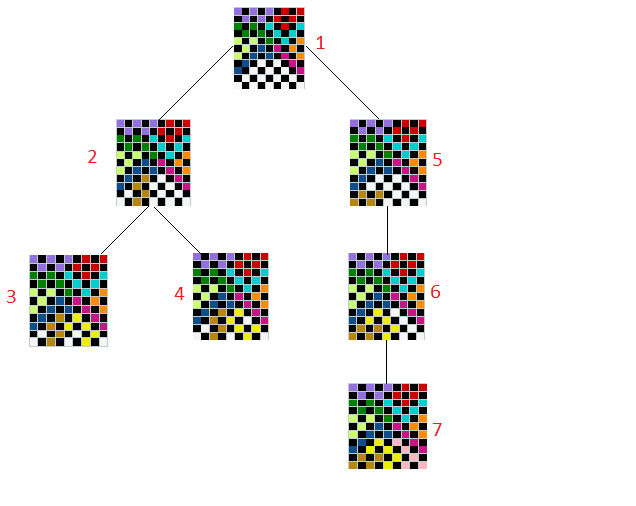
\includegraphics[scale=1]{immagini/0}
	\caption{Esempio di funzionamento dell'algoritmo DFS}
	\label{fig:0}
\end{figure}

\section{CSP}
\subsection{Descrizione}
Il secondo approccio utilizzato per risolvere questo gioco è stato formalizzare il problema in forma di CSP (Constraint Satisfaction Problem). Un CSP è composto da un insieme di variabili $X = \{X\textsubscript{1},...,X\textsubscript{n}\}$, i loro domini  $D = \{D\textsubscript{1},...,D\textsubscript{n}\}$ e un insieme di vincoli  $C = \{C\textsubscript{1},...,C\textsubscript{m}\}$, dove ogni vincolo coinvoge un sottoinsieme di variabili, specificandone una combinazione di valori permessi.\\
Uno stato è rappresentato da un assegnamento di valori ad alcune delle variabili $\{X\textsubscript{i} = v\textsubscript{i}, X\textsubscript{j} = v\textsubscript{j},...\}$.
Un assegnamento che non viola nessun vincolo è chiamato consistente, mentre un assegnamento dove ogni variabile ha un valore è detto completo. \\
La soluzione per un CSP è un assegnamento consistente e completo.

\subsection{Utilizzo}
Nella nostra implementazione il CSP è così definito:
\begin{itemize}
	\item \textbf{variabili}: tutte le forme, univocamente identificate dal loro colore;
	\item \textbf{domini}: l'insieme di valori validi per ogni variabile, dove un valore è una tupla di coordinate che identifica un possibile posizionamento di una forma nella griglia;
	\item \textbf{vincoli}: 
		\begin{itemize}
			\item nessuna variabile $X\textsubscript{i}$ deve sovrapporsi all'interno della griglia, anche solo parzialmente, con un'altra variabile $X\textsubscript{j}$;
			\item il posizionamento di una variabile nella griglia non deve creare una componente connessa con un numero di celle inferiore alla dimensione della forma più piccola, 3 nel nostro caso (vedi Figura \ref{fig:badCC}).
		\end{itemize}
\end{itemize}


\begin{figure}[h]
	\centering
	{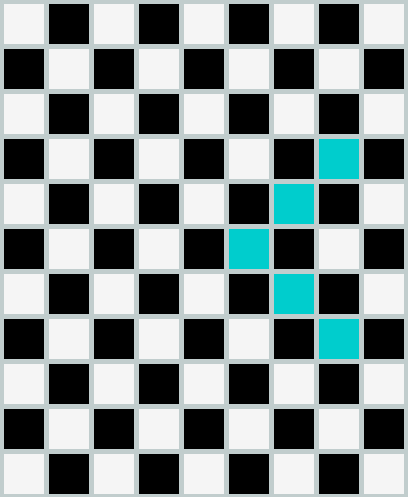
\includegraphics[scale=0.35]{immagini/goodCC}}
	\hspace{5mm}
	{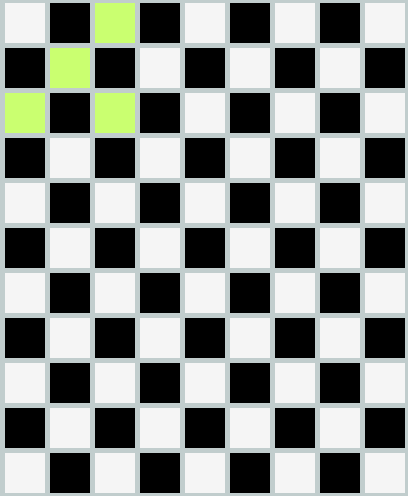
\includegraphics[scale=0.35]{immagini/badCC}}
	\caption{La figura a sinistra rappresente un valore consistente per la forma a "V", mentre la figura a destra uno non valido per la figura a "T" in quanto si crea una componente connessa di una sola cella}
	\label{fig:badCC}
\end{figure}

\subsection{Tipi di solver}
La libreria \textit{python-constraint} che abbiamo utilizzato per risolvere il problema sotto forma di CSP, mette a disposizione tre diversi solver, che utilizzano algoritmi ed euristiche differenti per ottenere una soluzione. \\
Inoltre abbiamo incluso e modificato il codice della libreria all'interno del nostro progetto per poter visualizzare nella griglia grafica ogni passo di computazione dei vari solver e aggiungere alcune migliorie esposte in \ref{migliorie}.
\subsubsection{Backtracking}
Questo solver ad ogni passo di computazione seleziona la prossima variabile a cui assegnare un valore attraverso l'euristica di grado, cioè per ogni variabile conta il numero di vincoli in cui è coinvolta, selezionando quella più vincolata. Qualora questa euristica evidenzi più di una variabile, a queste viene applicata l'euristica Minimum Remaining Values (MRV), che seleziona la variabile con il minor numero di valori nel dominio.\\
Una volta scelta la variabile le viene assegnato un valore consistente con l'assegnamento parziale, se esiste, eliminando dai domini delle altre variabili, attraverso un \textit{forward checking}, i valori non più consistenti con il nuovo assegnamento. Se non esiste un valore consistente nel dominio della variabile, si ritorna all'ultima variabile assegnata, cambiandone il valore. \\
Quando tutte le variabili hanno un valore nell'assegnamento, esso viene ritornato come soluzione del problema.
\subsubsection{Backtracking ricorsivo}
Utilizza lo stesso algoritmo esposto nel paragrafo precedente, solamente che viene implementato in modo ricorsivo.
\subsubsection{MinConflict}
Questo solver utilizza un algoritmo di ricera locale cioè, partendo da un assegnamento completo delle varibili, cerca di ottenere una soluzione al problema modificando ad ogni passo il valore di una variabile, facendo in modo che violi il minor numero di vincoli del problema. \\
Questi tipi di algoritmi non considerano il percorso per raggiungere una soluzione, ma danno importanza solamente alla configurazione finale. Inoltre utilizzando un unico stato corrente, possono portare alla soluzione utilizzando poca memoria, e spesso si rivelano più efficienti nel caso di un grande spazio degli stati, rispetto ad altri algoritmi.\\

\begin{figure}[h]
	\centering
	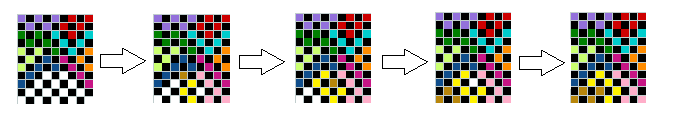
\includegraphics[scale=0.75]{immagini/mc}
	\caption{Funzionamento del solver MinConflict (da notare che alcune forme sono sovrapposte e quindi non del tutto visibili)}
	\label{fig:mc}
\end{figure}


\newpage
\section{Nostri miglioramenti}
\label{migliorie}
Una volta implementati gli algoritmi appena visti, abbiamo pensato a dei modi per poter miglorare la loro efficienza rispetto al nostro gioco. \\

\subsection{Connected Component Check}
Per quanto rigurda DFS, Backtracking e Backtracking ricorsivo abbiamo aggiunto un particolare controllo, se voluto dall'utente attraverso uno specifico input, chiamato \textbf{Connected Component Check}.
Durante l'esecuzione dei vari algoritmi, nel momento in cui viene deciso un valore per la prossima variabile da assegnare, insieme all'assegnamento parziale ottenuto fino a quel momento, viene fatto un controllo sulla dimensione della minima componente connessa rimanente nella griglia. \\
Se essa ha una dimensione minore della più piccola forma ancora da inserire, viene scartato il nuovo valore che si stava assegnando alla variabile e ne viene analizzato un altro. 

\begin{figure}[h]
	\centering
	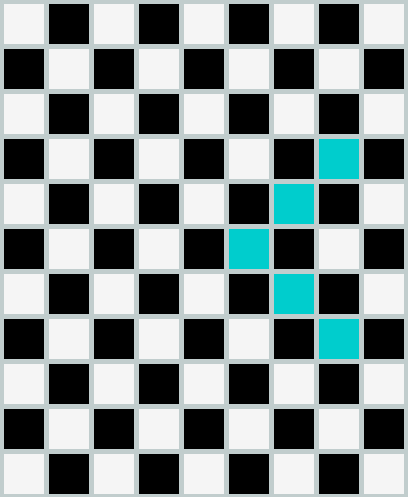
\includegraphics[scale=0.25]{immagini/goodCC}
	\caption{Assegnamento consistente per la variabile "V"}
	\label{fig:CCC}
\end{figure}

\begin{figure}[h]
	\centering
	{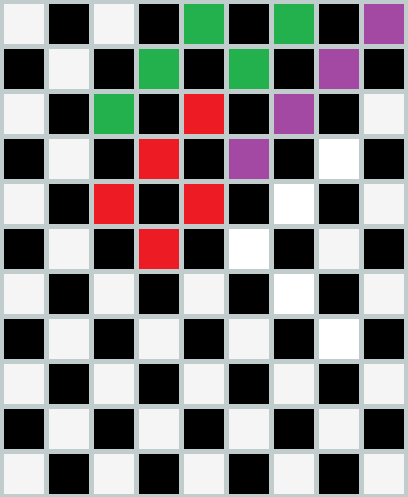
\includegraphics[scale=0.35]{immagini/esCC}}
	\hspace{5mm}
	{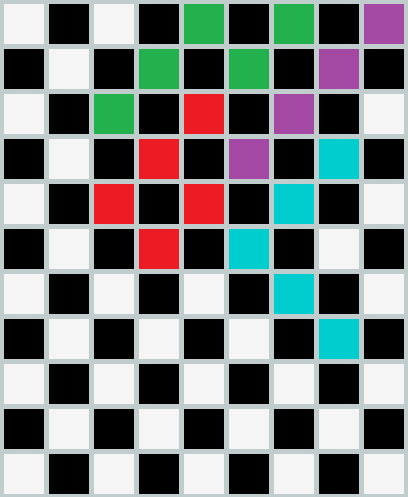
\includegraphics[scale=0.35]{immagini/esCC_no}}
	\caption{La stessa posizione della figura \ref{fig:CCC} per la variabile "V" non è consistente con l'assegnamento parziale, e l'algoritmo che fa uso di Connected Component Check è in grado di rilevarlo}
	\label{fig:badCCC}
\end{figure}

\subsection{Random Restart}
Abbiamo notato come il solver MinConflict nelle istanze complesse del problema non raggiunga un assegnamento completo e consistente, ossia una soluzione. Questo è dovuto dal fatto che può capitare di raggiungere stati dove ogni possibile successiva azione non diminuisce il numero di vincoli violati. Nel caso in cui l'algoritmo arrivi in uno di questi stati, chiamati minimi locali, non è più in grado di raggiungere una soluzione del problema, in quanto inizia una serie di assegnamenti ciclici che lo porteranno sempre allo stesso minimo locale, terminando dopo un numero fissato di iterazioni in un assegnamento non consistente.\\
Per ovviare a questo problema l'utente ha la possibilità, tramite uno specifico input nella definizione del problema, di utilizzare la tecnica chiamata Random Restart. Essa consiste nel riavviare l'algoritmo qualora termini con un assegnamento non consistente, finchè non ritorna una soluzione valida per il problema. Questa tecnica rende MinConflict completo, in quanto ci assicura di ottenere sempre un assegnamento completo e consistente, dopo un certo numero di riavvii.\\



              % Processi
% !TEX encoding = UTF-8
% !TEX TS-program = pdflatex
% !TEX root = ../tesi.tex

%**************************************************************
\chapter{Performance}
\label{cap:performance}
%**************************************************************
\section{Confronto dei vari metodi}
In questa sezione confronteremo il tempo di esecuzione dei vari metodi risolutivi per 5 configurazioni iniziali del problema, di difficoltà crescente dal livello 0 al livello 4.\\
Per i primi 4 problemi abbiamo anche un dato del tempo impiegato da un essere umano nel risolvere il problema (sezione \ref{human}). Abbiamo infatti sottoposto i vari livelli a 8 persone diverse, di età compresa tra 16 e 55 anni, cronometrandoli durante lo svolgimento del gioco.\\
Per ogni livello è presente una tabella che contiene le misure di performance, in termini di tempo medio di esecuzione, rilevate per ogni tipo di solver; inoltre tra parentesi è presente il numero medio di stati attraversati da ogni solver per arrivare allo stato obiettivo. \\
Per ogni tabella, si paragonano tra loro i risultati ottenuti da ogni solver con o senza le migliorie specificate in \ref{migliorie}

\section{Procedura di testing}
Per ogni livello di difficoltà e per ogni possibie algoritmo, con e senza le rispettive migliorie, sono state fatte 40 esecuzioni. Per ogni esecuzione sono stati tracciati il tempo e il numero di stati attraversati, per poi calcolare le medie da inserire nelle varie tabelle.\\
Nel caso del solver $MinConflict$ senza \textit{Random Restart}, i dati sono relativi alle sole esecuzioni che hanno portato ad una soluzione valida (le percentuali di fallimento/successo vengono riportate tra le osservazioni per ogni livello).

\newpage

\subsection{Livello 0}

La configurazione iniziale del livello 0 è mostrata in figura \ref{lev0}. Le forme mancanti da inserire sono mostrate nelle figure \ref{z}, \ref{c}, \ref{y}.
\begin{figure}[h]
	\centering
	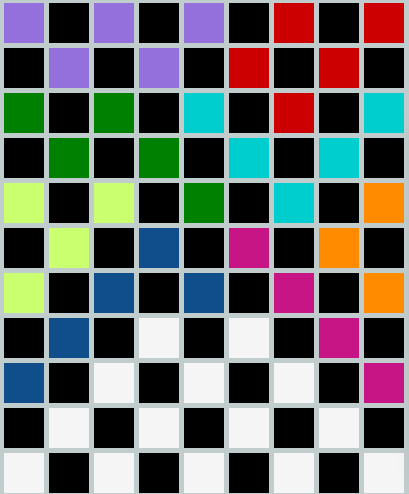
\includegraphics[scale=0.3]{immagini/lv0}
	\caption{Livello 0}
	\label{lev0}
\end{figure}
\\
\noindent

\begin{table}[h]
	\begin{tabular}{|l||*{4}{c|}}\hline 
		\backslashbox{Miglioria}{Solver} 
		&\makebox{DFS}&\makebox{Backtracking}&\makebox{Recursive Backtracking}	&\makebox{MinConflict}\\ \hline 
		Sì&\textcolor{ForestGreen}{0,0107 (4,175)}&\textcolor{red}{0,0519 (11)}&0,0495 (11)&0,0184 (2,275) \\ \hline 
		No&0,0319 (24,825)&0,0178 (11)&0,0175 (11)&0,0223 (2,525)  \\ \hline 
	\end{tabular} 
	\caption{Tempi livello 0}
\end{table}

\subsubsection{Osservazioni}
\label{oss0}
\textit{Numero di soluzioni}: 2\\

In questo livello, le forme mancanti sono solamente tre, producendo così uno spazio degli stati molto limitato. Secondo i test effettutati e sulla base delle misure di perfomance adottate ed esposte in \ref{performance}, l'algoritmo migliore risulta essere $DFS$ con la miglioria \textit{Connected Component Check} (d'ora in avanti $CCC$), mentre il peggiore risulta essere quello di $Backtracking$ con la stessa miglioria.\\

La miglioria $CCC$ permette a $DFS$ di ignorare una considerevole porzione dello spazio degli stati. Ipotizziamo di volere inserire la prima delle tre forme mancanti, creando una componente connessa di grandezza minore della più piccola forma ancora da inserire. Senza la miglioria, l'inserimento di tale forma produrrà un assegnamento parziale dal quale non è possibile raggiungere una configurazione finale che corrisponda ad un assegnamento totale e consistente, portando quindi $DFS$ ad esplorare totalmente un cammino che è destinato a non portare ad uno stato obiettivo.\\
La miglioria, invece, si accorgerebbe subito di questo problema evitando di assegnare quel valore alla variabile, potando il conseguente sottoalbero degli stati; infatti $DFS$ con miglioria attraversa in media 4,175 stati, mentre senza di essa ne attraversa in media 24,825, oscillando tra un minimo di 10 e un massimo di 30 stati.\\
Notiamo tuttavia che il tempo per arrivare alla soluzione da parte dei due tipi di $DFS$ non è proporzionale rispetto al numero degli stati attraversati (il primo numero di stati è $1/6$ dell'altro, mentre il primo tempo d'esecuzione è $1/3$ dell'altro). Questo è dovuto al fatto che il $CCC$ richiede ovviamente anch'esso un certo tempo di esecuzione (asintoticamente  $\mathcal{O}(n + m)$, dove $n$ è il numero di nodi e $m$ il numero di archi, se interpretiamo la griglia come un grafo), che però risulta vantaggioso ai fini dell'esplorazione dello spazio degli stati e della soluzione.\\

Per quanto riguarda il $Backtracking$ con la stessa miglioria, esso risulta essere il peggiore per il seguente motivo: notiamo come il $Backtracking$ semplice impieghi poco più del $DFS$ con miglioria, facendo quindi pensare che anch'esso sia un buon solver per questo livello di difficoltà. Tuttavia, dalla tabella si vede come il solver $Backtracking$ semplice e quello con miglioria attraversino lo stesso numero di stati, con la differenza che nel secondo viene eseguito il $CCC$, aumentandone quindi il tempo d'esecuzione.\\
Possiamo quindi affermare che a parità di stati, o se la loro differenza è poco rilevante, il solver che utilizza il $CCC$ impiegherà più tempo rispetto al suo corrispondente solver senza il $CCC$.\\

Infine, osserviamo che la miglioria \textit{Random Restart} per il solver $MinConflict$ risulta poco utile, in quanto per la semplicità di questo livello è molto difficile che il solver si "incastri" in qualche minimo locale: nessuno dei test eseguiti per questo solver, con e senza miglioria, ha mai portato ad uno stallo in un minimo locale e quindi i due solver operano allo stesso modo (non ci sono riavvii).
\newpage
\subsection{Livello 1}
La configurazione iniziale del livello 1 è mostrata in figura \ref{lev1}. Le forme mancanti da inserire sono mostrate nelle figure \ref{z}, \ref{c}, \ref{y}, \ref{w}.
\begin{figure}[h]
	\centering
	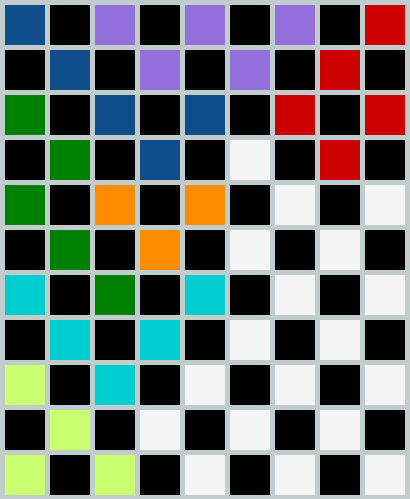
\includegraphics[scale=0.3]{immagini/lv1}
	\caption{Livello 1}
	\label{lev1}
\end{figure}
\\
\noindent
\begin{table} [h]
	\begin{tabular}{|l||*{4}{c|}}\hline 
		\backslashbox{Miglioria}{Solver} 
		&\makebox{DFS}&\makebox{Backtracking}&\makebox{Recursive Backtracking}	&\makebox{MinConflict}\\ \hline 
		Sì&\textcolor{ForestGreen}{0,0271 (9,75)}&0,0666 (12)&0,0704 (12)&\textcolor{red}{0,7078 (409,92)} \\ \hline 
		No&0,1081 (94,675)&0,0257 (12)&0,0270 (13)&0,0539 (10,518)  \\ \hline 
	\end{tabular} 
	\caption{Tempi livello 1}
\end{table}

\subsubsection{Osservazioni}

\textit{Numero di soluzioni}: 1\\

Per questo livello di difficoltà, i risultati ottenuti con i solver $DFS$, $Backtracking$ e \textit{Recursive Backtracking} rispecchiano quelli ottenuti nel livello 0. Non verrano quindi esposte altre osservazioni su questi solver, in quanto identiche a quelle del livello precedente.\\


Risulta invece necessario approfondire il significato dei valori riguardanti il solver $MinConflict$ (rimandiamo a \ref{RR} per il significato di miglioria in questo contesto).\\
Nonostante questo livello di difficoltà possa sembrare ancora semplice, il solver \textit{MinConflict} senza la miglioria \textit{Random Restart} (d'ora in avanti $RR$) non ha portato ad una soluzione nel $32,5\%$ dei test, risultando quindi di utilizzo scarsamente conveniente. \\
Con la miglioria $RR$, invece, vediamo come il tempo di esecuzione (e il numero di stati attraversati) sia nettamente più alto rispetto a qualsiasi altro solver, in quanto l'alto tasso di fallimento comporta spesso un numero elevato di riavvii dell'algoritmo. \\Tuttavia risulta che il numero di stati attraversati oscilli tra un minimo di 2 e un massimo di 5.006 (che corrispondono a 5 riavvii), con una maggior concentrazione intorno ai 20 stati. Quest'ultimo dato ci porta quindi a dedurre che è più probabile che il numero di stati attraversati sia circa 20, e non diverse migliaia.\\
Comunque sia, il solver $MinConflict$ resta il peggiore per questo livello.


\subsection{Livello 2}
La configurazione iniziale del livello 2 è mostrata in figura \ref{lev2}. Le forme mancanti da inserire sono mostrate nelle figure \ref{p}, \ref{smallv}, \ref{bigz}, \ref{i}, \ref{w}, \ref{v}.
\begin{figure}[h]
	\centering
	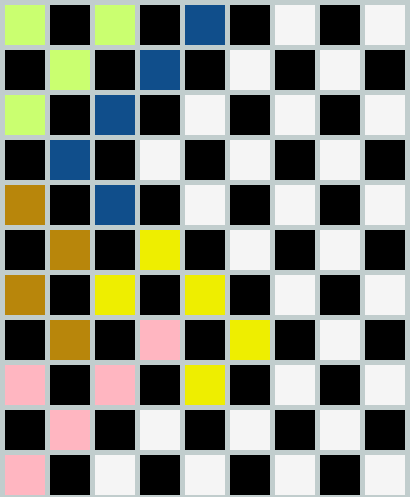
\includegraphics[scale=0.3]{immagini/lv2}
	\caption{Livello 2}
	\label{lev2}
\end{figure}
\\
\noindent
\begin{table}[h]
	\begin{tabular}{|l||*{4}{c|}}\hline 
		\backslashbox{Miglioria}{Solver} 
		&\makebox{DFS}&\makebox{Backtracking}&\makebox{Recursive Backtracking}	&\makebox{MinConflict}\\ \hline 
		Sì&0,1429 (57,75)&0,1405 (22)&0,1227 (17)&0,4244 (180,47) \\ \hline 
		No&\textcolor{red}{1,9350 (1901,25)}&0,0695 (32)&\textcolor{ForestGreen}{0,0579 (19)}&0,1850 (52,894)  \\ \hline 
	\end{tabular} 
	\caption{Tempi livello 2}
\end{table}

\subsubsection{Osservazioni}

\textit{Numero di soluzioni}: 8\\

In questo livello di difficoltà, il numero di forme da inserire è 6, generando così uno spazio degli stati notevolmente maggiore dei livelli precedentemente affrontati, con conseguenti osservazioni differenti.
Il solver migliore risulta infatti essere il \textit{Recursive Backtracking} senza il $CCC$, mentre il peggiore è il $DFS$ senza $CCC$, come ci si poteva attendere.\\

Osserviamo che $DFS$ senza $CCC$ risulta essere nettamente peggiore del suo corrispettivo con $CCC$: il tempo di esecuzione è infatti quasi 14 volte maggiore, mentre il numero di stati attraversati è circa 33 volte maggiore.\\

Per quanto riguarda il solver \textit{Recursive Backtracking} senza il $CCC$, osserviamo che non differisce di molto dal $Backtracking$ senza la stessa miglioria (infatti i tempi sono simili). Mentre essi necessitano molto più tempo per arrivare alla soluzione, se utilizzati con il $CCC$, per il motivo già spiegato nel Livello 0.\\

Le osservazioni per $MinConflict$ risultano essere le stesse del Livello 1, ma con parametri differenti: il solver senza il $RR$ è fallito solo nel $5\%$ dei test, mentre il solver con il $RR$ attraversa un numero di stati che oscilla da un minimo di 2 ad un massimo di 1.124. Il motivo per il quale la percentuale di fallimento è così bassa, rispetto al livello precedente, è che questa configurazione iniziale presenta 8 possibili diverse soluzioni.
\subsection{Livello 3}
La configurazione iniziale del livello 3 è mostrata in figura \ref{lev3}. Le forme mancanti da inserire sono mostrate nelle figure \ref{z}, \ref{smallv}, \ref{bigz}, \ref{c}, \ref{y}, \ref{t}, \ref{w}, \ref{v}.
\begin{figure}[h]
	\centering
	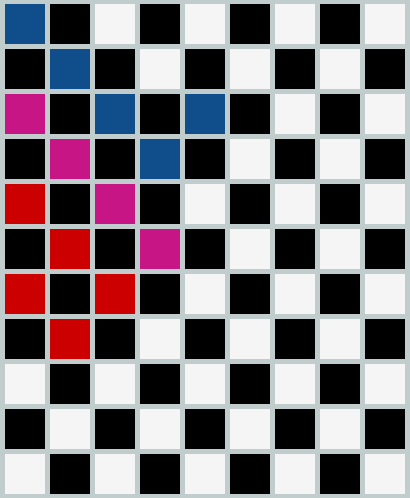
\includegraphics[scale=0.3]{immagini/lv3}
	\caption{Livello 3}
	\label{lev3}
\end{figure}
\\
\noindent

\begin{table}[h] 
	\begin{tabular}{|l||*{4}{c|}}\hline 
		\backslashbox{Miglioria}{Solver} 
		&\makebox{DFS}&\makebox{Backtracking}&\makebox{Recursive Backtracking}	&\makebox{MinConflict}\\ \hline 
		Sì&27,913 (8.750,4)&1,0607 (198)&\textcolor{ForestGreen}{0,3522 (55)}&32,192 (15.323) \\ \hline 
		No& \textcolor{red}{30 minuti}&1,0379 (1.179)&0,5709 (572)&2,56 (857)  \\ \hline 
	\end{tabular} 
	\caption{Tempi livello 3}
\end{table}

\subsubsection{Osservazioni}

\textit{Numero di soluzioni}: 1\\

Il livello 3 è il primo che presenta un grado di difficoltà elevato. Infatti il solver $DFS$ senza il $CCC$ impiega in media 30 minuti per arrivare ad una soluzione, ed è proprio in questo livello che si può meglio apprezzare l'utilità del $CCC$: il $DFS$ che fa utilizzo di tale miglioria impiega infatti solo 27 secondi in media per ottenere una soluzione.\\
Il solver dalle migliori prestazioni per questo problema è il \textit{Recursive Backtracking} con il $CCC$.\\

Nel solver $MinConflict$ i dati evidenziano invece che il solver senza $RR$ è parecchio veloce, ma porta ad una soluzione solo nel $2,5\%$ dei casi.
Con il $RR$, osserviamo che sono attraversati in media 15.323 stati (che corrispondono a 15 riavvii). Tuttavia questo numero oscilla da un minimo di 926 ad un massimo di 72.354 (72 riavvii).
Quest'ultimo dato ci fa capire che, per questo livello, affidarsi a questo solver è un azzardo spesso fallimentare: è molto difficile che porti ad una soluzione, oppure potrebbe metterci un tempo troppo elevato. 
\subsection{Livello 4}
La configurazione iniziale del livello 4 è mostrata in figura \ref{lev4}. Tutte le forme devono essere inserite nella griglia.
\begin{figure}[h]
	\centering
	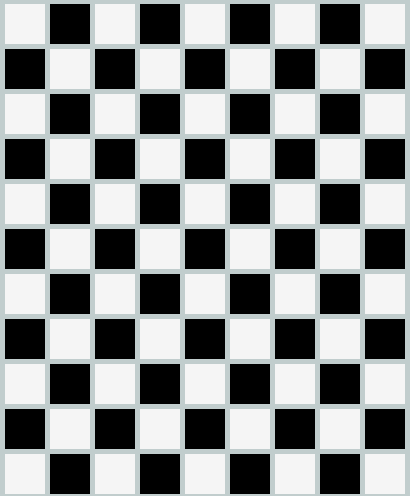
\includegraphics[scale=0.3]{immagini/lv4}
	\caption{Livello 4}
	\label{lev4}
\end{figure}
\\
\noindent

 \begin{table}[h] 
	\begin{tabular}{|l||*{4}{c|}}\hline 
		\backslashbox{Miglioria}{Solver} 
		&\makebox{DFS}&\makebox{Backtracking}&\makebox{Recursive Backtracking}	&\makebox{MinConflict}\\ \hline 
		Sì&\textcolor{red}{228,63 (77.582)}&\textcolor{ForestGreen}{1,0781 (184)}&13,126 (2.640)&18,794 (3.416,8) \\ \hline 
		No& ()&3,8761 (4.002)&23,131 (23.971)&2,94 (458,78)  \\ \hline 
	\end{tabular} 
	\caption{Tempi livello 4}
\end{table}

\subsubsection{Osservazioni}

\textit{Numero di soluzioni}: 2248\\

In quest'ultimo livello, il solver miglior è il $Backtracking$ con il $CCC$, mentre qualsiasi tipo di $DFS$ è ritenuto inaccettabile nel tempo di esecuzione.\\

Le osservazioni per $MinConflict$ risultano leggermente differenti dal Livello 3: il solver senza il $RR$ ha avuto successo nel $22,5\%$ dei test, mentre il solver con il $RR$ attraversa un numero di stati che oscilla da un minimo di 62 ad un massimo di 12.220 (12 riavvii), con una concentrazione tra i 3000 e i 6000 stati attraversati.\\
Il numero molto elevato di soluzioni possibili fa si che non siano necessari molti riavvii per questo livello, cosa che invece non accade nel livello 3.

\section{Prestazioni essere umano}
\label{human}
I dati raccolti, sottoponendo i primi 4 livelli (da 0 a 3) a 8 persone, sono raccolti nella seguente tabella (dati in secondi).


\begin{table}[h]
	\centering
	\begin{tabular}{lllll}
		\hline
		\multicolumn{1}{|c|}{Livelli}     & \multicolumn{1}{c|}{0}     & \multicolumn{1}{c|}{1}    & \multicolumn{1}{c|}{2}      & \multicolumn{1}{c|}{3}           \\ \hline
		\multicolumn{1}{|c|}{Tempo medio} & \multicolumn{1}{c|}{33,87} & \multicolumn{1}{c|}{35,8} & \multicolumn{1}{c|}{163,36} & \multicolumn{1}{c|}{39,7 minuti} \\ \hline                               
	\end{tabular}
	\caption{Tempi essere umano}
\end{table}
Questi risultati ci fanno capire la difficoltà presente in questo gioco, in particolar modo con l'aumentare del numero di forme da inserire. Questo è quindi un'ulteriore esempio di come l'intelligenza artificiale è in grado di risolvere relatiamente velocemente problemi che per l'uomo sarebbero intrattabili in tempi ragionevoli. 
             % Kick-Off
% !TEX encoding = UTF-8
% !TEX TS-program = pdflatex
% !TEX root = ../tesi.tex

%**************************************************************
\chapter{Conclusioni}
\label{cap:conclusioni}
%**************************************************************

\part{title}             % Concept Preview

%**************************************************************
% Materiale finale
%**************************************************************
\backmatter
\end{document}
